%\part*{Lezione 22/04/2021}
\newpage
\section{Biciclo CN-NO}\index{Ciclo CNNO@Ciclo CN-NO}\label{sec-CNNO}
Nelle stelle come il Sole (popolazione I) l'abbondanza di metalli è tale che i protoni possono reagire in elio con un processo diverso dalla catena $pp$\index{Catena protone-protone@Catena protone-protone $pp$}.
\begin{figure}[!h]
	\centering
	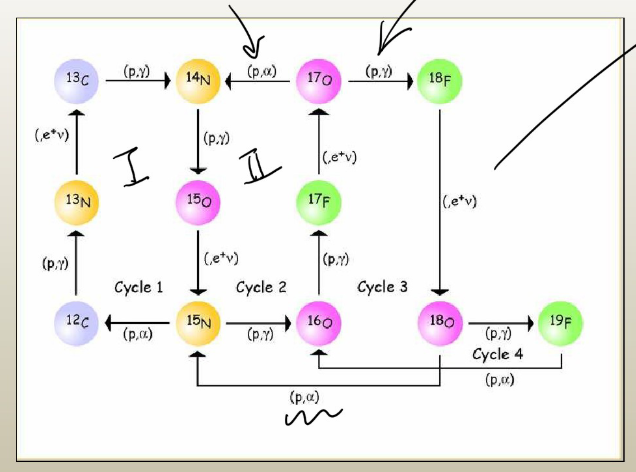
\includegraphics[scale=0.6]{Immagini/0422_CNO-complete-scheme.png}
	\caption{Schema completo del biciclo CN-NO}
	\label{0422_completescheme}
\end{figure}

\subsection{Ciclo CNO}
\begin{figure}[!h]
	\centering
	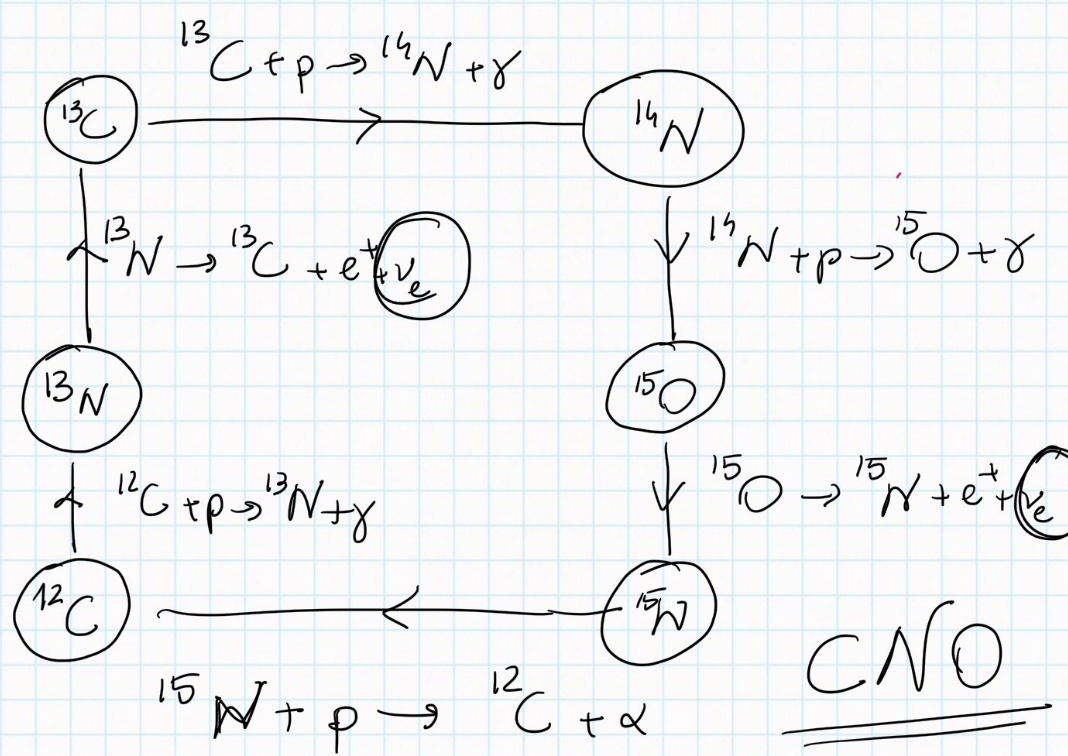
\includegraphics[scale=0.5]{Immagini/0422_CNOscheme.png}
	\caption{Schema del ciclo CNO.}
	\label{0422_CNOsch}
\end{figure}
$$\ce{^{12}C}(\textcolor{red}{p},\gamma)\ce{^{13}N}(e^+\nu_e)\ce{^{13}C}(\textcolor{red}{p},\gamma)\ce{^{14}N}(\textcolor{red}{p},\gamma)\ce{^{15}O}(e^+\nu_e)\ce{^{15}N}(\textcolor{red}{p},\textcolor{blue}{\alpha})\ce{^{12}C}$$
\noindent Come suggerisce il nome, non si tratta di una catena ma di un ciclo: si parte da $4p$ e si producono $\alpha + 2 e^+ + 2 \nu_e$ con $Q=26.7$ MeV, ristabilendo le condizioni per far ripartire il network di reazioni (i cosidetti \textit{seed}, ovvero $\ce{^{12}C}$ e $\ce{^{13}N}$, non si esauriscono).\\ 
Vediamo in Figura \ref{0422_sunCNO} che in base alla temperatura interna della stella il ciclo è più o meno dominante rispetto alla catena $pp$. Anche questa volta, per studiare questo network di reazioni si osservano i neutrini ($\nu_{\mbox{O}}$ e $\nu_{\mbox{N}}$), i cui flussi comparivano nella Figura \ref{0322_nu} (quando abbiamo studiato quelli della $pp$), e le rispettive reazioni hanno tempi di decadimento pari a $\tau_{\mbox{O}} \sim 2$ m e $\tau_{\mbox{N}} \sim 10$ m.

\begin{figure}[!h]
	\centering
	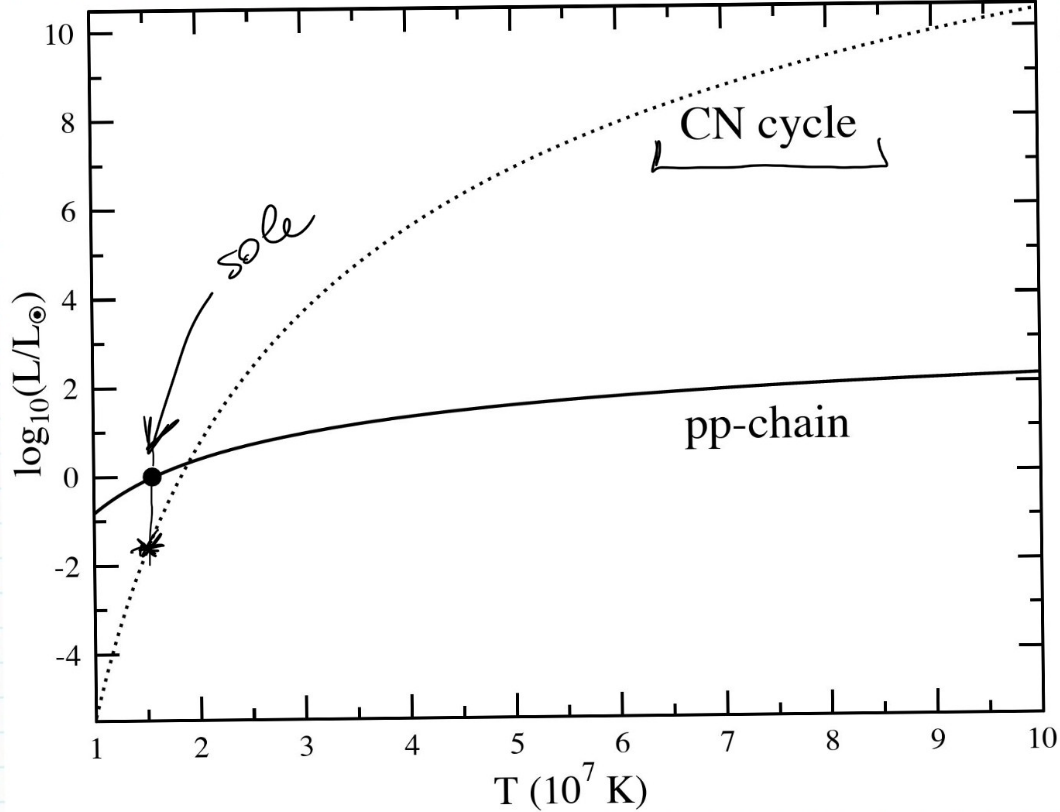
\includegraphics[scale=0.5]{Immagini/0422_CNO-pp.png}
	\caption{Contibuto della catena $pp$ e del ciclo CNO alla luminosità al variare della temperatura interna della stella. Il punto indica la posizione del Sole.}
	\label{0422_sunCNO}
\end{figure}

\paragraph{Un po' di notazione} Prima di studiare il network introduciamo una notazione per scrivere il reaction rate dei vari processi in gioco. Finora abbiamo visto:
\begin{align*}
	&1+2 \to \dots	& r_{12} &= \frac{n_1n_2}{1+\delta_{12}}\,\mean{\sigma v}_{12} \\
	&1\to \dots	& r_1 &= \lambda_1 n_1
\end{align*}
\noindent dove $\lambda \equiv 1/\tau$ è la costante di decadimento. Definiamo allora i fattori combinatoriali\index{fattori combinatoriali}:
\begin{align*}
	C_{ij} &= \frac{1}{1+\delta_{ij}}\:\longleftarrow \text{ numero di coppie distinte} & r_{ij} &= C_{ij}\, n_in_j\,\mean{\sigma v}_{ij} \\ 
	C_{ijk} &= \Biggl \{%
	\begin{array}{ll}
		1    & i,j,k \text{ diversi}\\
		1/2! & \forall\, i=j, j=k, i=k \\ 
		1/3! & i=j=k
	\end{array}%
	& r_{ijk} &= C_{ijk}\, n_in_j n_k\,\mean{\sigma v}_{ijk}
\end{align*}
\noindent Attraverso questi possiamo riscrivere la variazione nel tempo di densità di specie $i$ (equazione di rate) come:
\begin{align*}
	\tderpar{n_i} &= \sum_j r_j + \sum_{jk} r_{jk} + \sum_{jk\ell}  r_{jk\ell} = \\
	&= \sum_j  \lambda_j n_j + \sum_{jk} C_{jk} \,n_jn_k\, \mean{\sigma v}_{jk} + \sum_{jk\ell} C_{jk\ell}\,n_jn_kn_\ell\,\mean{\sigma v}_{jk\ell}    
\end{align*} 
\noindent dove i termini con $j,k,\ell = i$ sono negativi (termini di distruzione) e viceversa quelli con $j,k,\ell \not = i$ (termini di creazione). Spesso questa relazione viene riscritta con la \textit{fractional nuclear abundance}\index{fractional nuclear abundance@\textit{fractional nuclear abundance}} $Y_i$, ovvero il numero di nuclei $i$ sul numero di nuclei totali, per cui\footnote{Se abbiamo una singola specie $Y=1/A$ e $n = \rho/Am_u = Y\rho/m_u$, per cui ricordandosi che il valore del numero d'Avogadro $N_u = 1/m_u$ si ha $n=\rho N_u Y$; generalizzando a più specie $n_i = \rho N_u Y_i$.} $\sum_i Y_i A_i = 1$:
$$\tderpar{Y_i} = \sum_j \lambda_j Y_j + \rho N_u\, \sum_{jk} C_{jk}\,Y_jY_k\, \mean{\sigma v}_{jk} + (\rho N_u)^2\,\sum_{jk\ell} C_{jk\ell}\,Y_jY_kY_\ell\,\mean{\sigma v}_{jk\ell} $$

\paragraph{Studio del network} 
Vediamo le reazioni che abbiamo:
\begin{enumerate}
	\item 3 reazioni $(p,\gamma)$ per $X = \ce{^{12}C},\ce{^{13}C},\ce{^{14}N}$, per le quali chiameremo $\mean{\sigma v} = \mean{\sigma v}_{p,X}$.
	\item 2 decadimenti $\beta^+$ per $X = \ce{^{14}N},\ce{^{15}O}$, per i quali definiamo $\lambda_X$.
	\item 1 reazione $(p,\alpha)$ per $\ce{^{15}N}$ e quindi $\mean{\sigma v}$.
\end{enumerate}
Riportiamo in Figura \ref{0422_reaz} la variazione nel tempo delle \textit{fractional nuclear abundance} per ogni specie; dalla fisica nulceare abbiamo ogni $\mean{\sigma v}$ e $\lambda$ e queste equazioni vengono risolte numericamente.

\begin{figure}[!h]
	\centering
	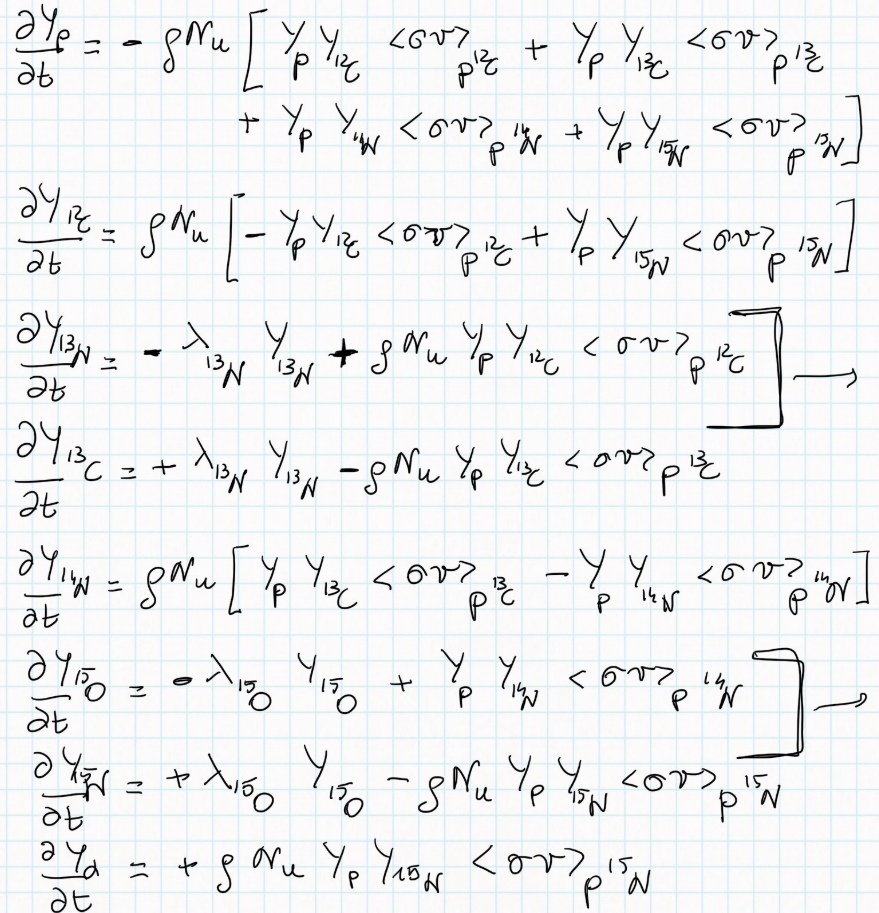
\includegraphics[scale=0.5]{Immagini/0422_reazioni.png}
	\caption{Evoluzione nel tempo per ogni specie.}
	\label{0422_reaz}
\end{figure}

\noindent Ci possiamo chiedere però quale tra queste sia la reazione più lenta. Abbiamo 2 processi deboli ($\ce{^{13}N}\to\ce{^{13}C}$ $\tau\sim 10$ min e $\ce{^{15}O}\to\ce{^{16}N}$ $\tau\sim 2$ min), ma nessuno dei due ha barriera coulombiana, quindi non sono i più lenti. La barriera è presente invece nei processi: $p+\ce{^{12}C}$, $p+\ce{^{13}C}$, $p+\ce{^{14}N}$ e $p+\ce{^{15}N}$; avendo l'azoto $Z=7$ maggiore di quello del carbonio $Z=6$, la barriera è più intensa per le reazioni con N e tra queste dal momento che $p+\ce{^{15}N}$ è un'interazione forte la più lenta è $p+\ce{^{14}N}$. Anche se sembra poco intuitivo i processi deboli raggiungono velocemente l'equilibrio (\textit{steady state}), $\partial_t Y =0$:
\begin{align*}
	\lambda_{\ce{^{13}N}} Y_{\ce{^{13}N}} &= \rho N_u Y_p Y_{\ce{^{12}C}} \, \mean{\sigma v}_{p\ce{^{12}C}} \\
	\lambda_{\ce{^{15}O}} Y_{\ce{^{15}O}} &= \rho N_u Y_p Y_{\ce{^{14}N}} \, \mean{\sigma v}_{p\ce{^{14}N}}	
\end{align*}
\noindent Sostituendo in Figura \ref{0422_reaz} e imponendo l'equilibrio di tutte le specie si ottiene:
$$\frac{Y_{\ce{^{14}N}}}{Y_{\ce{^{12}C}}} = \frac{\mean{\sigma v}_{p\ce{^{12}C}}}{\mean{\sigma v}_{p\ce{^{14}N}}} \simeq \frac{1.26 \cdot\ord{-12}\unit{cm}^3/\mbox{mol s}}{1.3 \cdot\ord{-14}\unit{cm}^3/\mbox{mol s}}\sim 100$$
Si intuisce quindi che al termine del ciclo anche se i \textit{seeds} sono ancora presenti, non hanno le stesse abbondanze iniziali, ma la maggior parte del carbonio\footnote{Vale anche per l'ossigeno.} viene processato e contribuisce ad aumentare l'abbondanza di azoto. Lo studio della reazione più lenta $\ce{^{14}N(p,\gamma)\ce{^{15}O}}$ diviene allora fondamentale per la stima delle abbondanze e dell'evoluzione stellare.

\subsection{Ciclo NO}
\begin{figure}[!h]
	\centering
	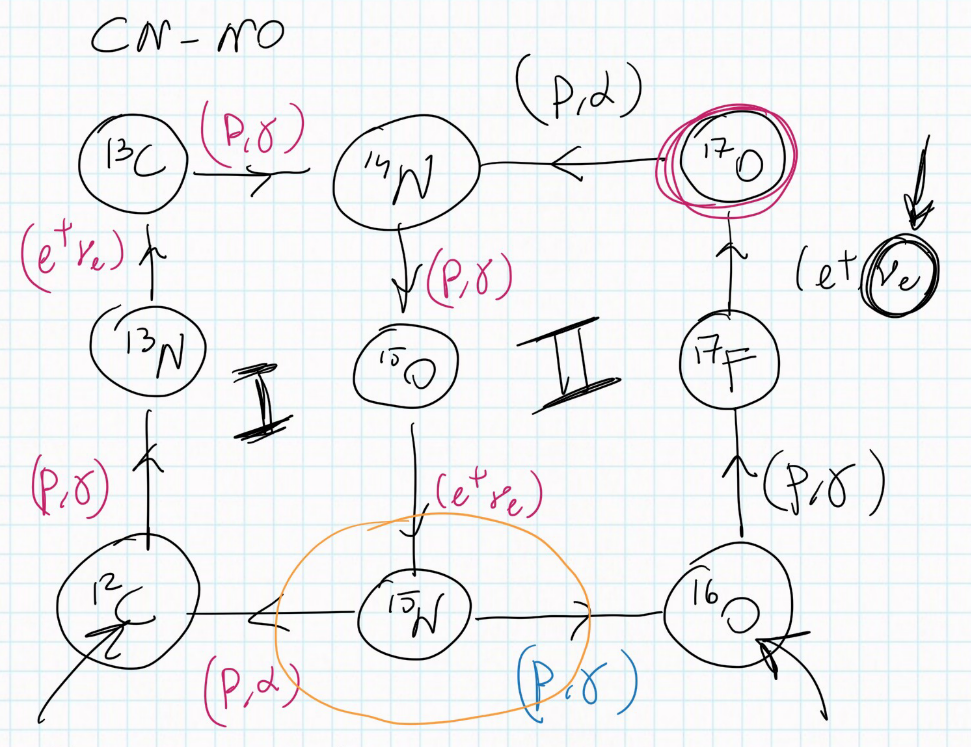
\includegraphics[scale=0.5]{Immagini/0422_biCNNOscheme.png}
	\caption{schema del biciclo CN-NO.}
	\label{0422_NO}
\end{figure}
$$\ce{^{14}N}(p,\gamma)\ce{^{15}O}(e^+\nu_e)\ce{^{15}N}(p,\gamma)\ce{^{16}O}(p,\gamma)\ce{^{16}O}(p,\gamma)\ce{^{17}F}(e^+\nu_e)\ce{^{17}O}(p,\alpha)\ce{^{14}N}$$
\acc{E} presente in realtà un secondo ciclo (da cui il nome biciclo) che coinvolge l'azoto e l'ossigeno (\textit{seed}); si può infatti avere, invece che $\ce{^{15}N}(p,\alpha)\ce{^{12}C}$, la reazione $\ce{^{15}N}(p,\gamma)\ce{^{16}O}$. Il rapporto tra i rate delle due reazioni è dato da\footnote{Cambiamo notazione dal momento che i reagenti sono gli stessi per le due reazioni; in questo caso vengono indicati i prodotti.}:
$$\frac{r_{p\alpha}}{r_{p\gamma}}\simeq \frac{\mean{\sigma v}_{p\alpha}}{\mean{\sigma v}_{p\gamma}}\sim\frac{S_{p\alpha}(0)}{S_{p\gamma}(0)}\simeq \frac{65\unit{MeV b}}{64\unit{keV b}}\sim 1000$$
Dunque, il secondo ciclo si accende circa ogni 1000 volte che si è completato il primo\footnote{Si può notare infatti che l'interazione della reazione che porta al primo ciclo è forte, mentre l'altra è elettromagnetica.}. Particolarmente importante per il rilevamento di questo network è il decadimento $\beta^+$ del $\ce{^{17}F}$ (neutrini $\nu_F$ come si vede in Figura \ref{0322_nu}).\\ 
Lo studio del biciclo CN-NO permette di determinare le abbondanze degli elementi C,N, O. 

\paragraph{Non solo due cicli}
Come si può notare in Figura \ref{0422_completescheme} sono presenti altri due cicli che si attivano con la reazione $\ce{^{17}O}(p,\gamma)\ce{^{18}F}$, ma questi riguardano stelle massicce le cui temperature interne superano le barriere di potenziale delle reazioni.

\subsection{La reazione più lenta}\label{sec-reaz-lenta}
\begin{figure}[!h]
	\centering
	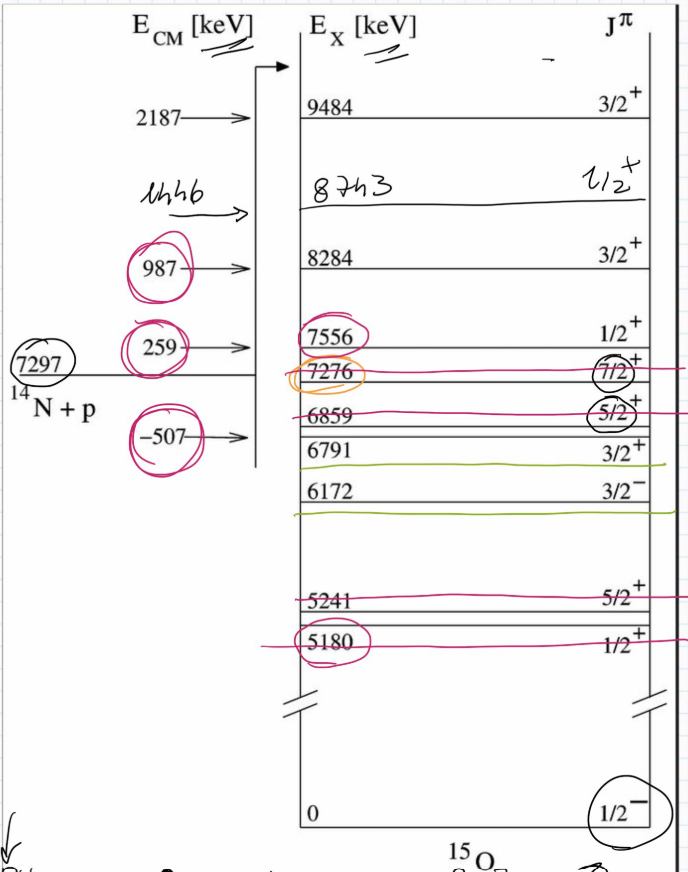
\includegraphics[scale=0.5]{Immagini/0422_lv-ene.png}
	\caption{Schema dei livelli energetici della reazione $\ce{^{14}N(p,\gamma)\ce{^{15}O}}$: 7297 keV è il $Q$-valore. I livelli sottolineati e cerchiati corrispondono alle risonanze, i livelli barrati sono risonanze trascurabili.}
	\label{0422_lv}
\end{figure}
\noindent Nel Sole (e in tutte le stelle di massa maggiore), come già detto, la reazione $\ce{^{14}N(p,\gamma)\ce{^{15}O}}$ è particolarmente importante sia per l'evoluzione che per la stima delle abbondanze dei \textit{seeds}. Riportiamo i livelli energetici del $\ce{^{15}O}$ in Figura \ref{0422_lv}. La finestra di Gamow è $30\div 110$ keV, per cui la risonanza $1/2^+$ a 5180 keV (lontana) non ci preoccupa; anche le risonanze con $J^\pi> 5/2$ data la multipolarità elevata non danno fastidio, mentre non possiamo trascurare la risonanza per $1/2^+$ (soprasoglia) e $3/2^\pm$ (risonanza sottosoglia) e la cattura diretta sul \textit{ground state} $1/2^-$. Sono state studiate in paricolar modo dall'esperimento LUNA\esperimento{LUNA}\footnote{Guarda \complrif{compl-multipoli}.}.

\begin{figure}[!h]
	\centering
	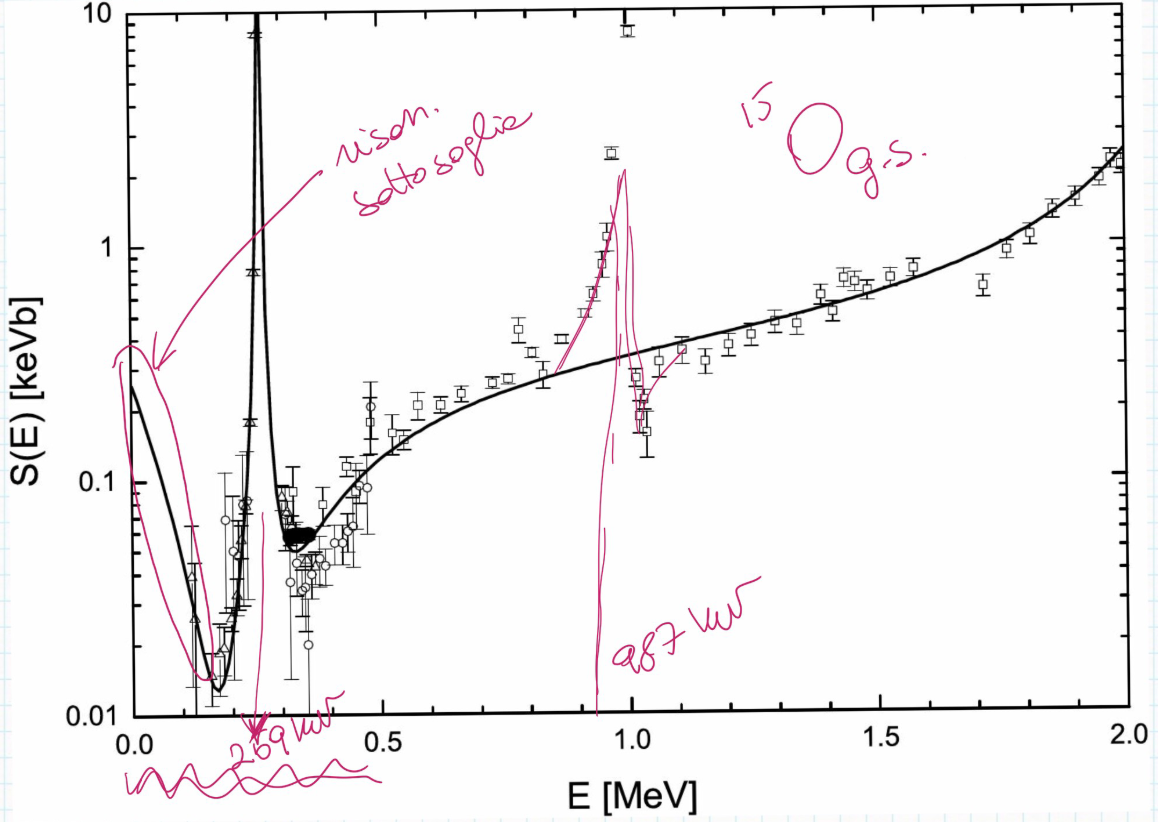
\includegraphics[scale=0.5]{Immagini/0422_0-Se.png}
	\caption{Fattore astrofisico per la cattura diretta sul fondamentale: la linea nera corrisponde al fit ottenuto con il metodo $R$-MATRIX.}
	\label{0422_cattura}
\end{figure}

\begin{itemize}
	\item \textbf{Cattura diretta}.Riportiamo in Figura \ref{0422_cattura} il fit eseguito con il metodo della $R$-MATRIX\index{metodo Rmatrix@metodo $R$-MATRIX}\footnote{Vedi il capitolo \secrif{sec-R-mat}.}. Osserviamo 3 risonanze, a 259 keV, a 987 keV e a 1446 keV (non di interesse), e una risonanza sottosoglia (a -507 keV); la multipolarità si distingue invece dalla distribuzione angolare. Si stima un fattore astrofisico: $$S(0)= (0.27\pm0.05) \unit{keV b}$$
	\item \textbf{Cattura $E_R=6.17\unit{MeV}$}. Il fattore astrofisico dello stato eccitato $3/2^-$ è rimportato in Figura \ref{0422_Er1} (fit con $R$-MATRIX). Si vedono le stesse 3 risonanze soprasoglia, ma non quella sottosoglia. Estrapolando dai dati: $$S_{6.17}(0)= (0.13\pm0.06) \unit{keV b}$$ I multipoli coinvolti sono $M1$ e $E2$. %
	\begin{figure}[!h]
		\centering
		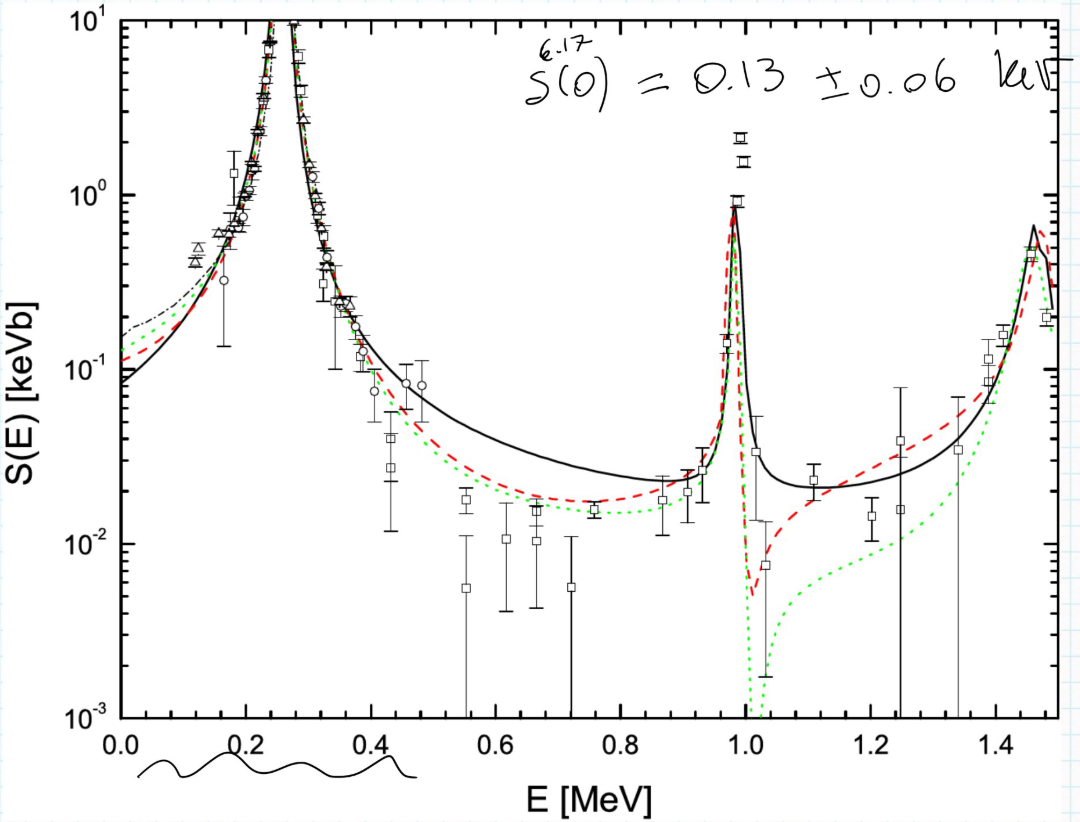
\includegraphics[scale=0.5]{Immagini/0422_0-Se-1.png}
		\caption{Fattore astrofisico per la cattura sullo stato risonante $E_R=6.17\unit{MeV}$: la linea nera corrisponde al fit ottenuto con il metodo $R$-MATRIX.}
		\label{0422_Er1}
	\end{figure}	
	\item \textbf{Cattura $E_R=6.79\unit{MeV}$}. I risultati per lo stato eccitato risonante $3/2^+$ sono riportati in Figura \ref{0422_Er2}. Il valore del fattore astrofisico così ottenuto è: $$S_{6.79}(0) = (1.18\pm 0.05)\unit{keV b}$$ Il multipolo coinvolto è $E1$.\\ Questo è il termine che dà il contributo maggiore al fattore astrofisco totale (misura di LUNA II\index{LUNA!LUNA II}): $$S_{tot}(0) = (1.66\pm 0.12)\unit{keV b}$$%
	\begin{figure}[!h]
		\centering
		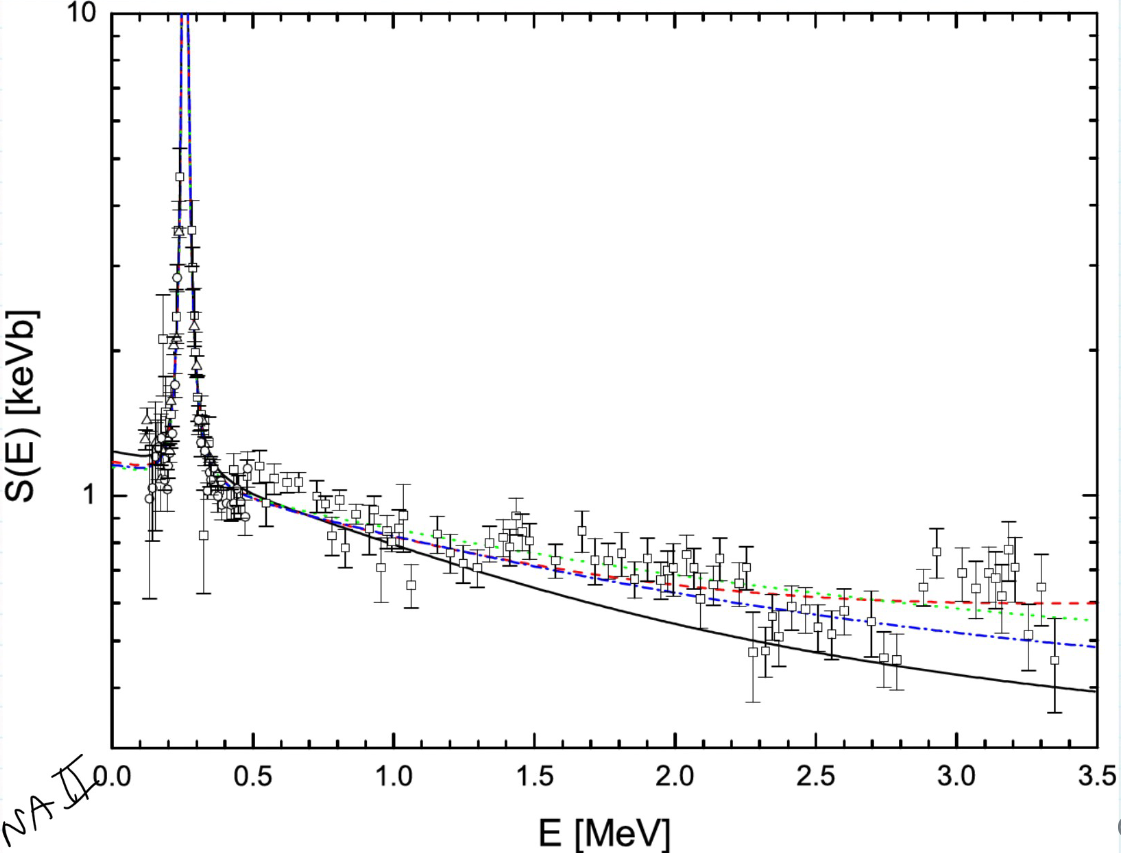
\includegraphics[scale=0.5]{Immagini/0422_0-Se-2.png}
		\caption{Fattore astrofisico per la cattura sullo stato risonante $E_R=6.79\unit{MeV}$: la linea nera corrisponde al fit ottenuto con il metodo $R$-MATRIX.}
		\label{0422_Er2}
	\end{figure}	
\end{itemize}

\paragraph{Un po' di storia}
Nel tempo si sono susseguiti diversi studi di questa reazione per stimarne il fattore astrofisico. 
\begin{itemize}
	\item 1988 - pochi dati che non permettevano di confermare o confutare la presenza della risonanza. Figura \ref{0422_19881998} a sinistra.
	\item 1998 - si ottiene un fit, ma le incertezze sono \vir{enormi}. Il fattore astrofisico così calcolatore fu:
	$$S(0)= \Bigl ( 3.5\begin{array}{l}
		+1.0 \\
		-2.0
	\end{array}%
	\Bigr )\unit{keV b}$$
	Figura \ref{0422_19881998} a destra. L'articolo\ di\ riferimento\ è\ Adelberger et al., Rev.\ Mod.\ Phys., 1998, vol.70, \texttt{DOI:}\doi{10.1103/RevModPhys.70.1265}.
	\item 2001 - viene introdotto il metodo $R$-MATRIX e si effettua un'analisi su dati precedenti, ottenendo così:
	$$S(0) = (1.77 \pm 0.20) \unit{keV b}$$
	Figura \ref{0422_2001}.
	\item Infine come abbiamo già visto LUNA II
\end{itemize}

\begin{figure}[!h]
	\centering
	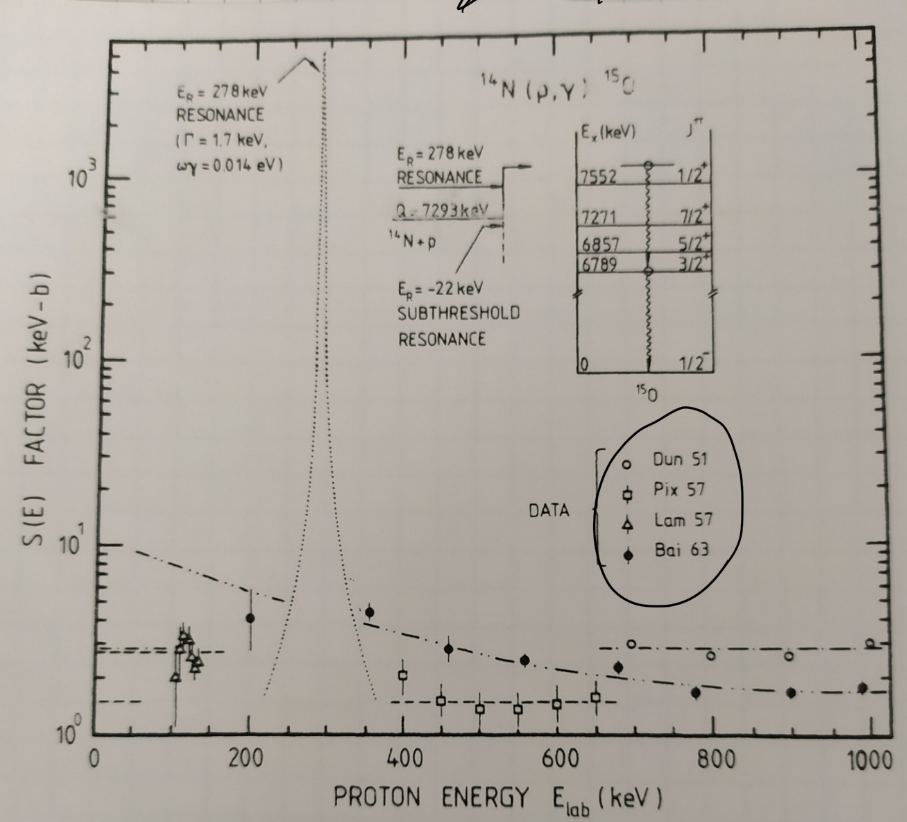
\includegraphics[scale=0.5]{Immagini/0422_Se.png}
	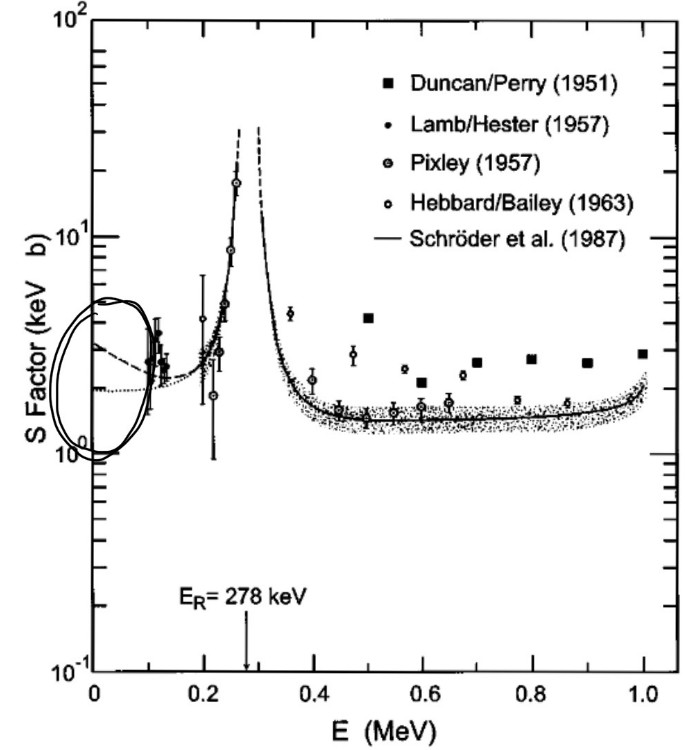
\includegraphics[scale=0.5]{Immagini/0422_Se2.png}
	\caption{A sinistra risultati del 1988.
	A destra risultati del 1998: la linea a puntini non tiene conto della risonanza sottosoglia, quella a tratti sì.}
	\label{0422_19881998}
\end{figure}

\begin{figure}[!h]
	\centering
	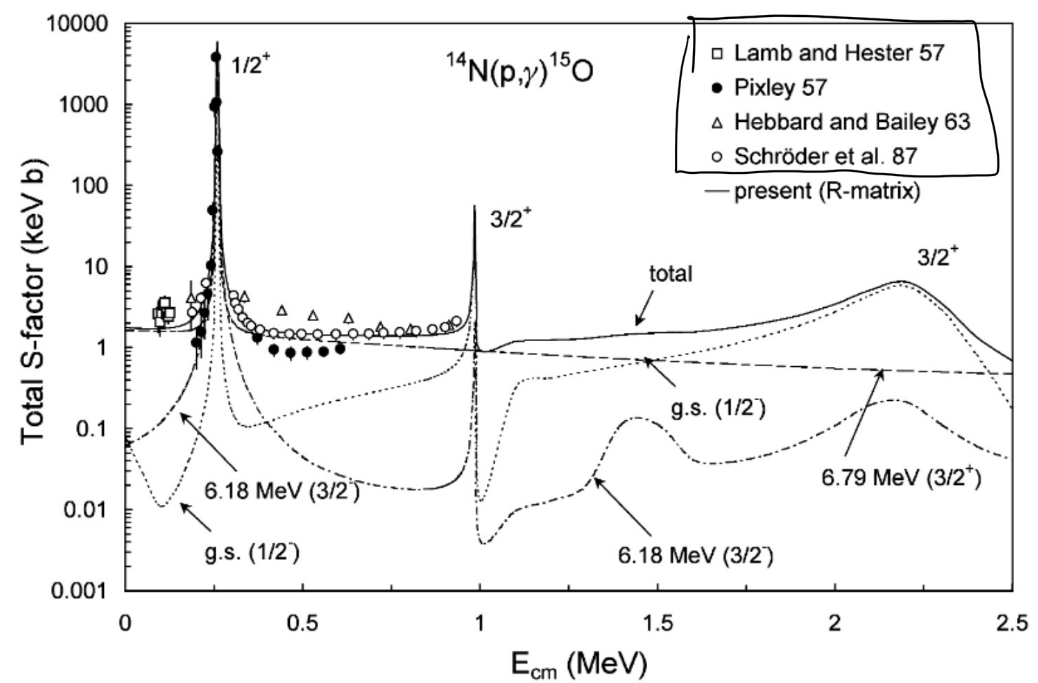
\includegraphics[scale=0.5]{Immagini/0422_Se3.png}
	\caption{Risultati del 2001.}
	\label{0422_2001}
\end{figure}






